\documentclass{standalone}
\usepackage{tikz}
\usetikzlibrary{patterns, positioning}
\usepackage[sfdefault]{ClearSans} %% option 'sfdefault' activates Clear Sans as the default text font
\usepackage[T1]{fontenc}

\begin{document}
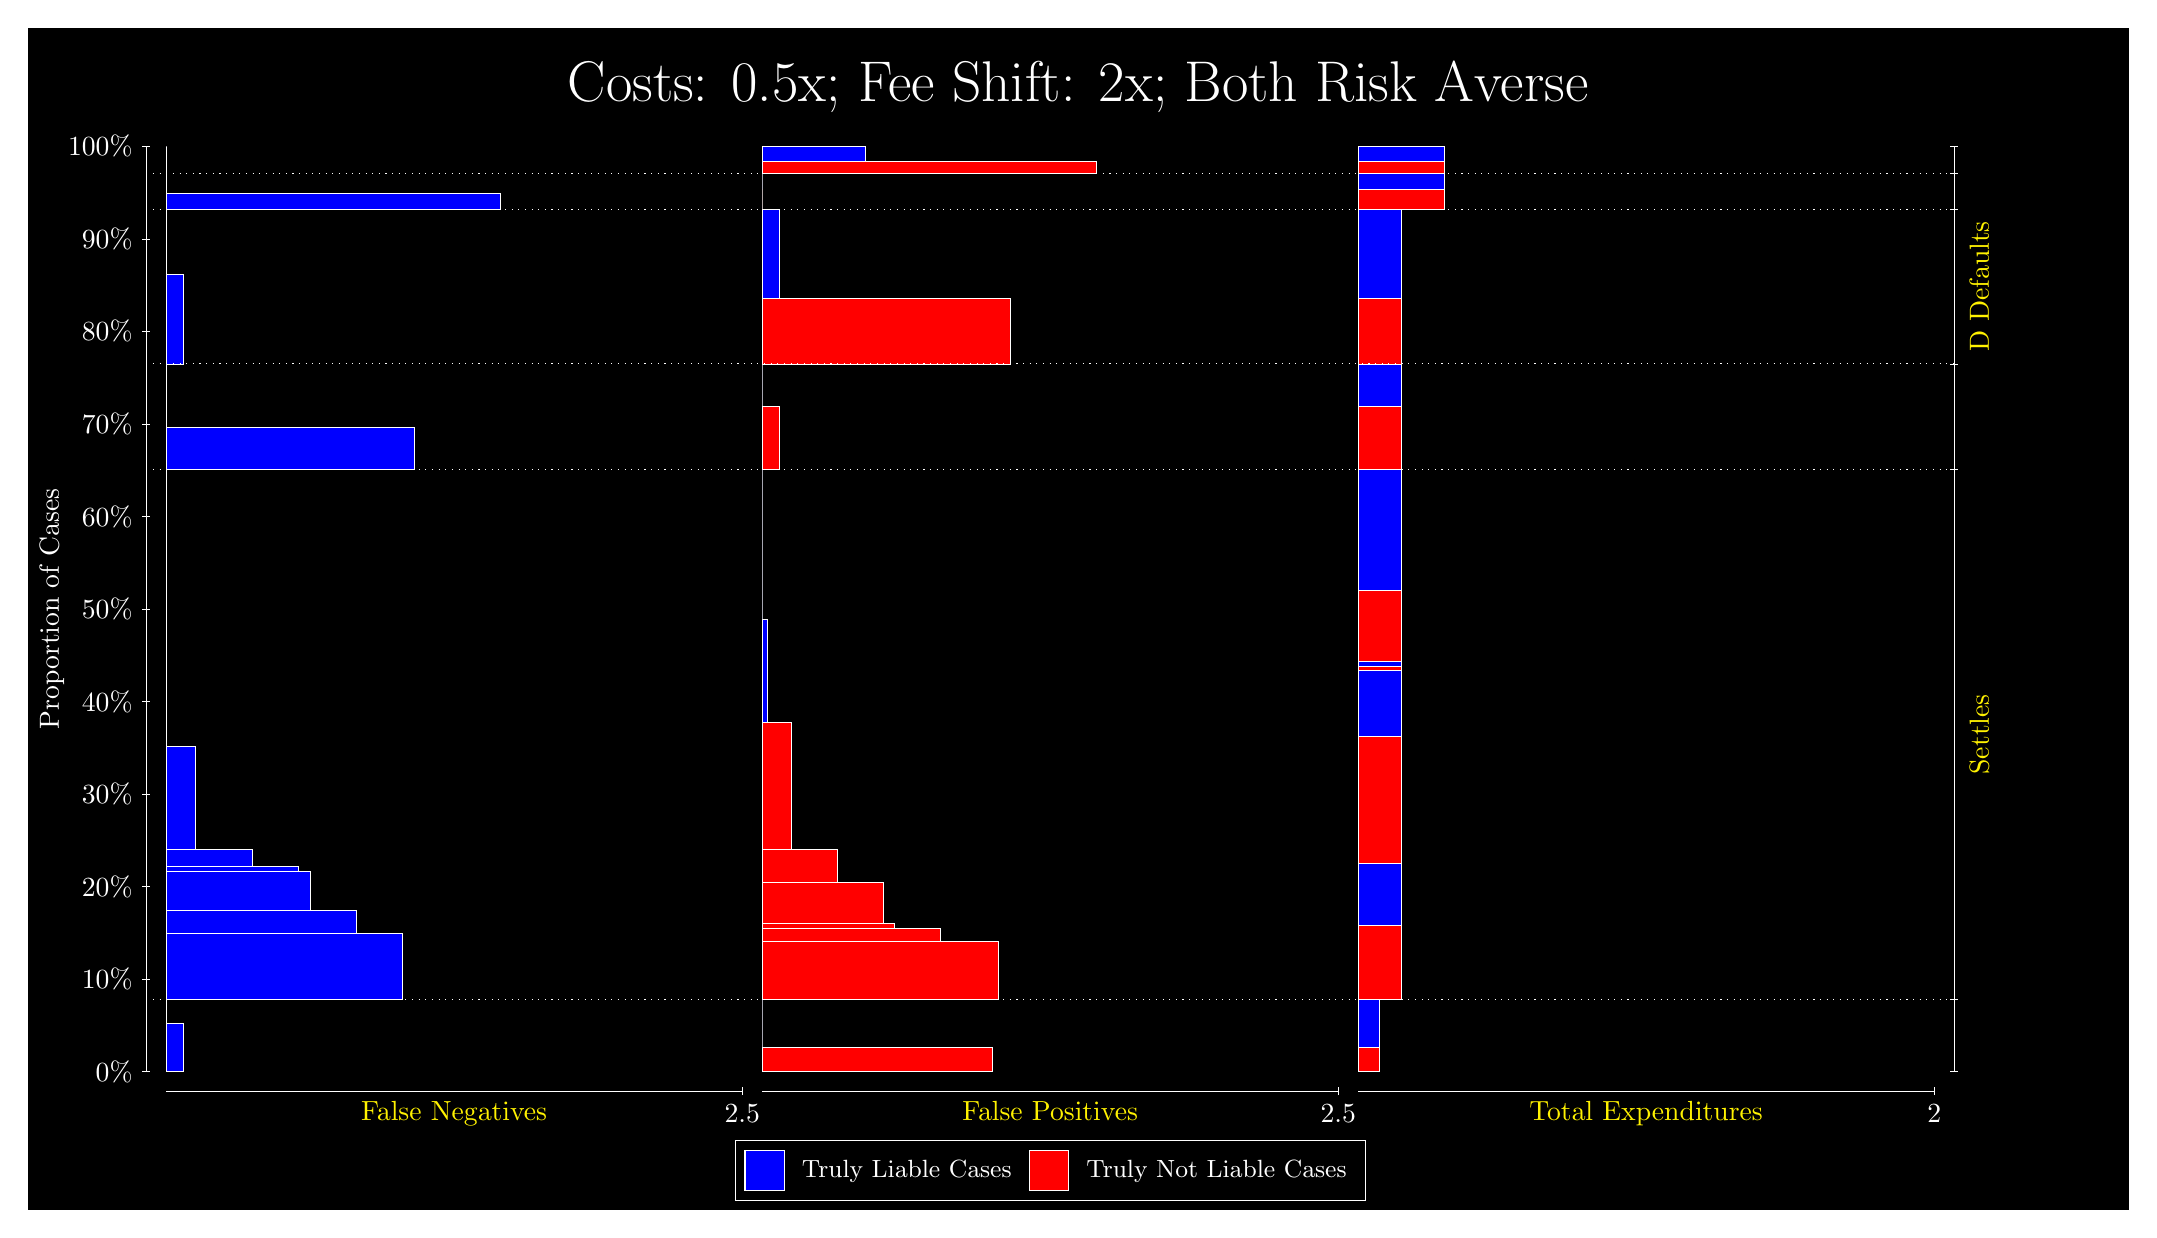
\begin{tikzpicture}
\draw[fill=black] (0,0) rectangle (26.667,15);
\draw[text=white] (0,13.5) rectangle (26.667,15) node[midway] {\huge Costs: 0.5x; Fee Shift: 2x; Both Risk Averse};
\draw[white, very thin] (1.5,1.75) -- (1.5,13.5);
\node[rotate=90, text=white, anchor=center] at (0.3, 7.625) {Proportion of Cases};
\draw[white, very thin] (1.45,1.75) -- (1.55,1.75);
\node[text=white, anchor=east] at (1.45, 1.75) {0\%};
\draw[white, very thin] (1.45,2.925) -- (1.55,2.925);
\node[text=white, anchor=east] at (1.45, 2.925) {10\%};
\draw[white, very thin] (1.45,4.1) -- (1.55,4.1);
\node[text=white, anchor=east] at (1.45, 4.1) {20\%};
\draw[white, very thin] (1.45,5.275) -- (1.55,5.275);
\node[text=white, anchor=east] at (1.45, 5.275) {30\%};
\draw[white, very thin] (1.45,6.45) -- (1.55,6.45);
\node[text=white, anchor=east] at (1.45, 6.45) {40\%};
\draw[white, very thin] (1.45,7.625) -- (1.55,7.625);
\node[text=white, anchor=east] at (1.45, 7.625) {50\%};
\draw[white, very thin] (1.45,8.8) -- (1.55,8.8);
\node[text=white, anchor=east] at (1.45, 8.8) {60\%};
\draw[white, very thin] (1.45,9.975) -- (1.55,9.975);
\node[text=white, anchor=east] at (1.45, 9.975) {70\%};
\draw[white, very thin] (1.45,11.15) -- (1.55,11.15);
\node[text=white, anchor=east] at (1.45, 11.15) {80\%};
\draw[white, very thin] (1.45,12.325) -- (1.55,12.325);
\node[text=white, anchor=east] at (1.45, 12.325) {90\%};
\draw[white, very thin] (1.45,13.5) -- (1.55,13.5);
\node[text=white, anchor=east] at (1.45, 13.5) {100\%};

\draw[white, very thin] (24.457,1.75) -- (24.457,13.5);
\draw[white, very thin] (24.407,1.75) -- (24.507,1.75);
\node[anchor=west] at (24.407, 1.75) {};
\draw[white, very thin] (24.407,2.6668) -- (24.507,2.6668);
\node[anchor=west] at (24.407, 2.6668) {};
\draw[white, very thin] (24.407,9.3972) -- (24.507,9.3972);
\node[anchor=west] at (24.407, 9.3972) {};
\draw[white, very thin] (24.407,10.738) -- (24.507,10.738);
\node[anchor=west] at (24.407, 10.738) {};
\draw[white, very thin] (24.407,12.701) -- (24.507,12.701);
\node[anchor=west] at (24.407, 12.701) {};
\draw[white, very thin] (24.407,13.152) -- (24.507,13.152);
\node[anchor=west] at (24.407, 13.152) {};
\draw[white, very thin] (24.407,13.5) -- (24.507,13.5);
\node[anchor=west] at (24.407, 13.5) {};

\draw[white, very thin, fill=blue] (1.75,1.75) rectangle (1.9696,2.3574);
\draw[white, very thin, fill=red] (1.75,2.3574) rectangle (1.75,2.6668);
\draw[white, very thin, fill=blue] (1.75,2.6668) rectangle (4.7507,3.5048);
\draw[white, very thin, fill=blue] (1.75,3.5048) rectangle (4.1652,3.801);
\draw[white, very thin, fill=blue] (1.75,3.801) rectangle (3.5797,4.294);
\draw[white, very thin, fill=blue] (1.75,4.294) rectangle (3.4333,4.3538);
\draw[white, very thin, fill=blue] (1.75,4.3538) rectangle (2.8478,4.5746);
\draw[white, very thin, fill=blue] (1.75,4.5746) rectangle (2.1159,5.883);
\draw[white, very thin, fill=red] (1.75,5.883) rectangle (1.75,9.3972);
\draw[white, very thin, fill=blue] (1.75,9.3972) rectangle (4.8971,9.9307);
\draw[white, very thin, fill=red] (1.75,9.9307) rectangle (1.75,10.738);
\draw[white, very thin, fill=blue] (1.75,10.738) rectangle (1.9696,11.874);
\draw[white, very thin, fill=red] (1.75,11.874) rectangle (1.75,12.701);
\draw[white, very thin, fill=blue] (1.75,12.701) rectangle (5.9949,12.898);
\draw[white, very thin, fill=red] (1.75,12.898) rectangle (1.75,13.152);
\draw[white, very thin, fill=red] (1.75,13.152) rectangle (1.75,13.316);
\draw[white, very thin, fill=blue] (1.75,13.316) rectangle (1.75,13.5);
\draw[white, very thin, fill=red] (9.3189,1.75) rectangle (12.246,2.0594);
\draw[white, very thin, fill=blue] (9.3189,2.0594) rectangle (9.3189,2.6668);
\draw[white, very thin, fill=red] (9.3189,2.6668) rectangle (12.32,3.3981);
\draw[white, very thin, fill=red] (9.3189,3.3981) rectangle (11.588,3.5721);
\draw[white, very thin, fill=red] (9.3189,3.5721) rectangle (11.002,3.6349);
\draw[white, very thin, fill=red] (9.3189,3.6349) rectangle (10.856,4.1549);
\draw[white, very thin, fill=red] (9.3189,4.1549) rectangle (10.27,4.5743);
\draw[white, very thin, fill=red] (9.3189,4.5743) rectangle (9.6848,6.181);
\draw[white, very thin, fill=blue] (9.3189,6.181) rectangle (9.3921,7.4894);
\draw[white, very thin, fill=blue] (9.3189,7.4894) rectangle (9.3189,9.3972);
\draw[white, very thin, fill=red] (9.3189,9.3972) rectangle (9.5384,10.204);
\draw[white, very thin, fill=blue] (9.3189,10.204) rectangle (9.3189,10.738);
\draw[white, very thin, fill=red] (9.3189,10.738) rectangle (12.466,11.565);
\draw[white, very thin, fill=blue] (9.3189,11.565) rectangle (9.5384,12.701);
\draw[white, very thin, fill=red] (9.3189,12.701) rectangle (9.3189,12.955);
\draw[white, very thin, fill=blue] (9.3189,12.955) rectangle (9.3189,13.152);
\draw[white, very thin, fill=red] (9.3189,13.152) rectangle (13.564,13.316);
\draw[white, very thin, fill=blue] (9.3189,13.316) rectangle (10.636,13.5);
\draw[white, very thin, fill=red] (16.888,1.75) rectangle (17.162,2.0594);
\draw[white, very thin, fill=blue] (16.888,2.0594) rectangle (17.162,2.6668);
\draw[white, very thin, fill=red] (16.888,2.6668) rectangle (17.437,3.6062);
\draw[white, very thin, fill=blue] (16.888,3.6062) rectangle (17.437,4.3955);
\draw[white, very thin, fill=red] (16.888,4.3955) rectangle (17.437,6.0021);
\draw[white, very thin, fill=blue] (16.888,6.0021) rectangle (17.437,6.8401);
\draw[white, very thin, fill=red] (16.888,6.8401) rectangle (17.437,6.9029);
\draw[white, very thin, fill=blue] (16.888,6.9029) rectangle (17.437,6.9627);
\draw[white, very thin, fill=red] (16.888,6.9627) rectangle (17.437,7.868);
\draw[white, very thin, fill=blue] (16.888,7.868) rectangle (17.437,9.3972);
\draw[white, very thin, fill=red] (16.888,9.3972) rectangle (17.437,10.204);
\draw[white, very thin, fill=blue] (16.888,10.204) rectangle (17.437,10.738);
\draw[white, very thin, fill=red] (16.888,10.738) rectangle (17.437,11.565);
\draw[white, very thin, fill=blue] (16.888,11.565) rectangle (17.437,12.701);
\draw[white, very thin, fill=red] (16.888,12.701) rectangle (17.986,12.955);
\draw[white, very thin, fill=blue] (16.888,12.955) rectangle (17.986,13.152);
\draw[white, very thin, fill=red] (16.888,13.152) rectangle (17.986,13.316);
\draw[white, very thin, fill=blue] (16.888,13.316) rectangle (17.986,13.5);
\draw[white, dotted] (1.5,2.6668) -- (24.457,2.6668);
\draw[white, dotted] (1.5,9.3972) -- (24.457,9.3972);
\draw[white, dotted] (1.5,10.738) -- (24.457,10.738);
\draw[white, dotted] (1.5,12.701) -- (24.457,12.701);
\draw[white, dotted] (1.5,13.152) -- (24.457,13.152);
\draw[white, very thin] (1.75,1.5) -- (9.0689,1.5);
\node[text=yellow, anchor=north] at (5.4094, 1.5) {False Negatives};
\draw[white, very thin] (9.0689,1.45) -- (9.0689,1.55);
\node[text=white, anchor=north] at (9.0689, 1.45) {2.5};

\draw[white, very thin] (9.3189,1.5) -- (16.638,1.5);
\node[text=yellow, anchor=north] at (12.978, 1.5) {False Positives};
\draw[white, very thin] (16.638,1.45) -- (16.638,1.55);
\node[text=white, anchor=north] at (16.638, 1.45) {2.5};

\draw[white, very thin] (16.888,1.5) -- (24.207,1.5);
\node[text=yellow, anchor=north] at (20.547, 1.5) {Total Expenditures};
\draw[white, very thin] (24.207,1.45) -- (24.207,1.55);
\node[text=white, anchor=north] at (24.207, 1.45) {2};


\node[text=yellow, centered, rotate=90] at (24.777, 6.032) {Settles};

\node[text=yellow, centered, rotate=90] at (24.777, 11.719) {D Defaults};



\draw (12.978300999999998,1.5) node[draw=none] (baseCoordinate) {};
\begin{scope}[align=center]
        \matrix[scale=0.5, draw=white, below=0.5cm of baseCoordinate, nodes={draw}, column sep=0.1cm]{
            \node[rectangle, draw, minimum width=0.5cm, minimum height=0.5cm, fill=blue] {}; &
            \node[draw=none, font=\small, text=white] (B) {Truly Liable Cases}; &
            \node[rectangle, draw, minimum width=0.5cm, minimum height=0.5cm, fill=red] {}; &
            \node[draw=none, font=\small, text=white] (B) {Truly Not Liable Cases}; \\
            };
\end{scope}

\end{tikzpicture}
\end{document}